\documentclass[11 pt]{article}
\pagenumbering{gobble}
\usepackage[bmargin=1in,tmargin=1in,lmargin=1.0in,rmargin=1.0in]{geometry}
\usepackage[dvipsnames]{xcolor}
\usepackage{amsfonts,amsmath,color,amssymb, url, enumerate, bbm}
\usepackage{pgfplotstable, pgfplots}
\usepackage{graphicx}
\usepackage{tikz}
\usepackage[title,titletoc]{appendix}
\usetikzlibrary{patterns, arrows}
\usepackage{subcaption}
\usepackage[noend]{algpseudocode}
\usepackage{algorithm}
\usepackage{float}
\usepackage{dashbox}
\pgfplotsset{compat=newest}
\usepackage{multicol}
\usepackage{hyperref}
\hypersetup{
    colorlinks=true,
    linkcolor=blue,
    filecolor=magenta,      
    urlcolor=blue,
}

\newtheorem{thm}{Theorem}[section]
\newtheorem{lm}{Lemma}[section]
\newtheorem{pf}{Proof}[section]
\newtheorem{defn}{Definition}[section]

\newcommand{\mcom}[1]{\marginpar{#1}}
\newcommand{\ilcom}[1]{\textcolor{red}{[#1]}}   
\newcommand{\dbbox}[1]{\dashbox{\textbf{#1}}}          

\title{ENGRI 1101 Software Installation}
\date{}

\usepackage{setspace}
\singlespacing
\begin{document}

\maketitle

\section{Anaconda Installation}

In this class, we will use a Python distribution called \href{https://www.anaconda.com/}{Anaconda}. More specifically, we will use the Individual Edition. First, download the \href{https://www.anaconda.com/products/individual}{Anaconda Graphical Installer}. Over the course of the semester, you will complete some labs in Jupyter Notebooks which allow you to run Python code. Many of these labs rely on various Python packages. A Python package is essentially pre-bundled code that serves some functionality. You will need to install the following packages. 

\begin{center}
\begin{tabular}{ll}
 \texttt{gilp} & Visualize the simplex algorithm and solve linear programs \\
 \texttt{ortools} & Google's optimization suite \\
 \texttt{networkx} &  Create and manipulate complex networks \\
 \texttt{matplotlib} & Publication quality figures in python \\
 \texttt{pandas} & High-performance, easy-to-use data structures and data analysis tools \\
 \texttt{bokeh} & Statistical and novel interactive html plots for python \\
 \texttt{shapely} & Manipulation and analysis of geometric objects in the cartesian plane \\
 \texttt{scipy} & Scientific library for python \\
 \texttt{scikit-image} & Image processing routines for scipy \\
 \texttt{numpy} & Array processing for numbers, strings, records, and objects \\
\end{tabular}
\end{center}

We will now walk through the steps for creating a virtual environment in Anaconda. In a virtual environment, the installed packages are isolated to that environment. Hence, if you install a python package in one environment, you could not reference it in another. After creating the virtual environment, we will install all the necessary packages for the semester. First, open up the Anaconda application.

\begin{enumerate}

\item Navigate to the \texttt{Environments} tab
\item Click create. You will get a pop-up like the one below. Name your environment \texttt{ENGRI\char`_1101} and use Python version 3.7

\begin{center}
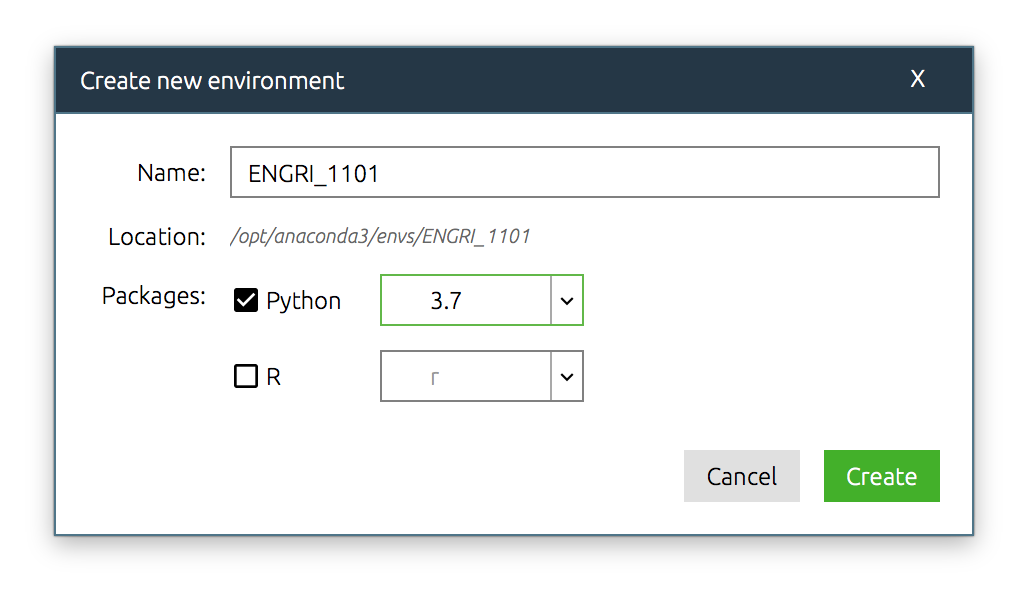
\includegraphics[scale=0.5]{create_env}
\end{center}

\item You should now see \texttt{ENGRI\char`_1101} in your list of environments. Click the play button and choose \texttt{Open Terminal}
\item Run the following line in the terminal that appears: $$\texttt{pip install gilp}$$
\item Wait for the install to complete and then run $$\texttt{pip install ortools}$$
\item Again, wait for the install to complete and then run $$\texttt{conda install -c conda-forge shapely}$$
\item Close the terminal window once the final installation is complete.
\item Go back to the \texttt{Environments} tab and change the list of packages from \texttt{Installed} to \texttt{Not installed}. Search for the remaining packages: \texttt{networkx}, \texttt{matplotlib}, \texttt{pandas},  \texttt{bokeh}, and  \texttt{scikit-image} and select them using the check box on the left.
\item Click \texttt{Apply} and you will see this pop-up. Make sure your pop-up contains all 5 packages in the red box. You will notice additional packages are also installed. These are dependencies of the 5 packages we really care about.

\begin{center}
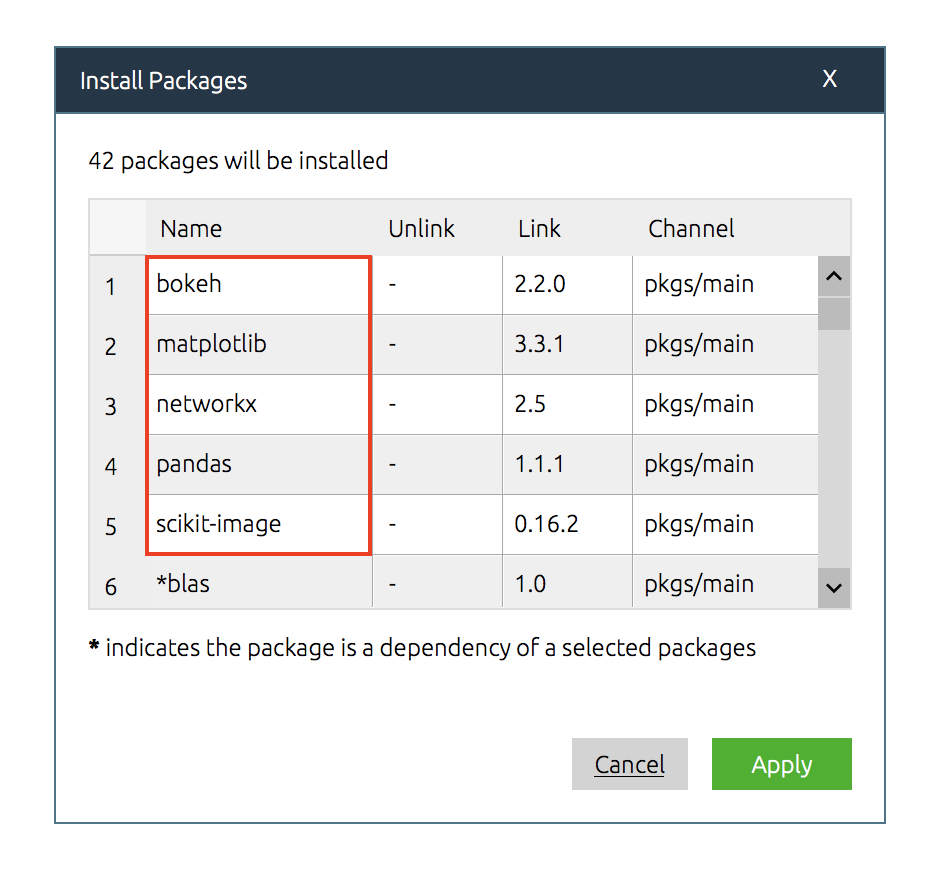
\includegraphics[scale=0.5]{package_installs}
\end{center}

\item Once the installation is complete, navigate back to the \texttt{Home} tab. Change the \texttt{Applications on} drop-down to your new \texttt{ENGRI\char`_1101} environment.

\begin{center}
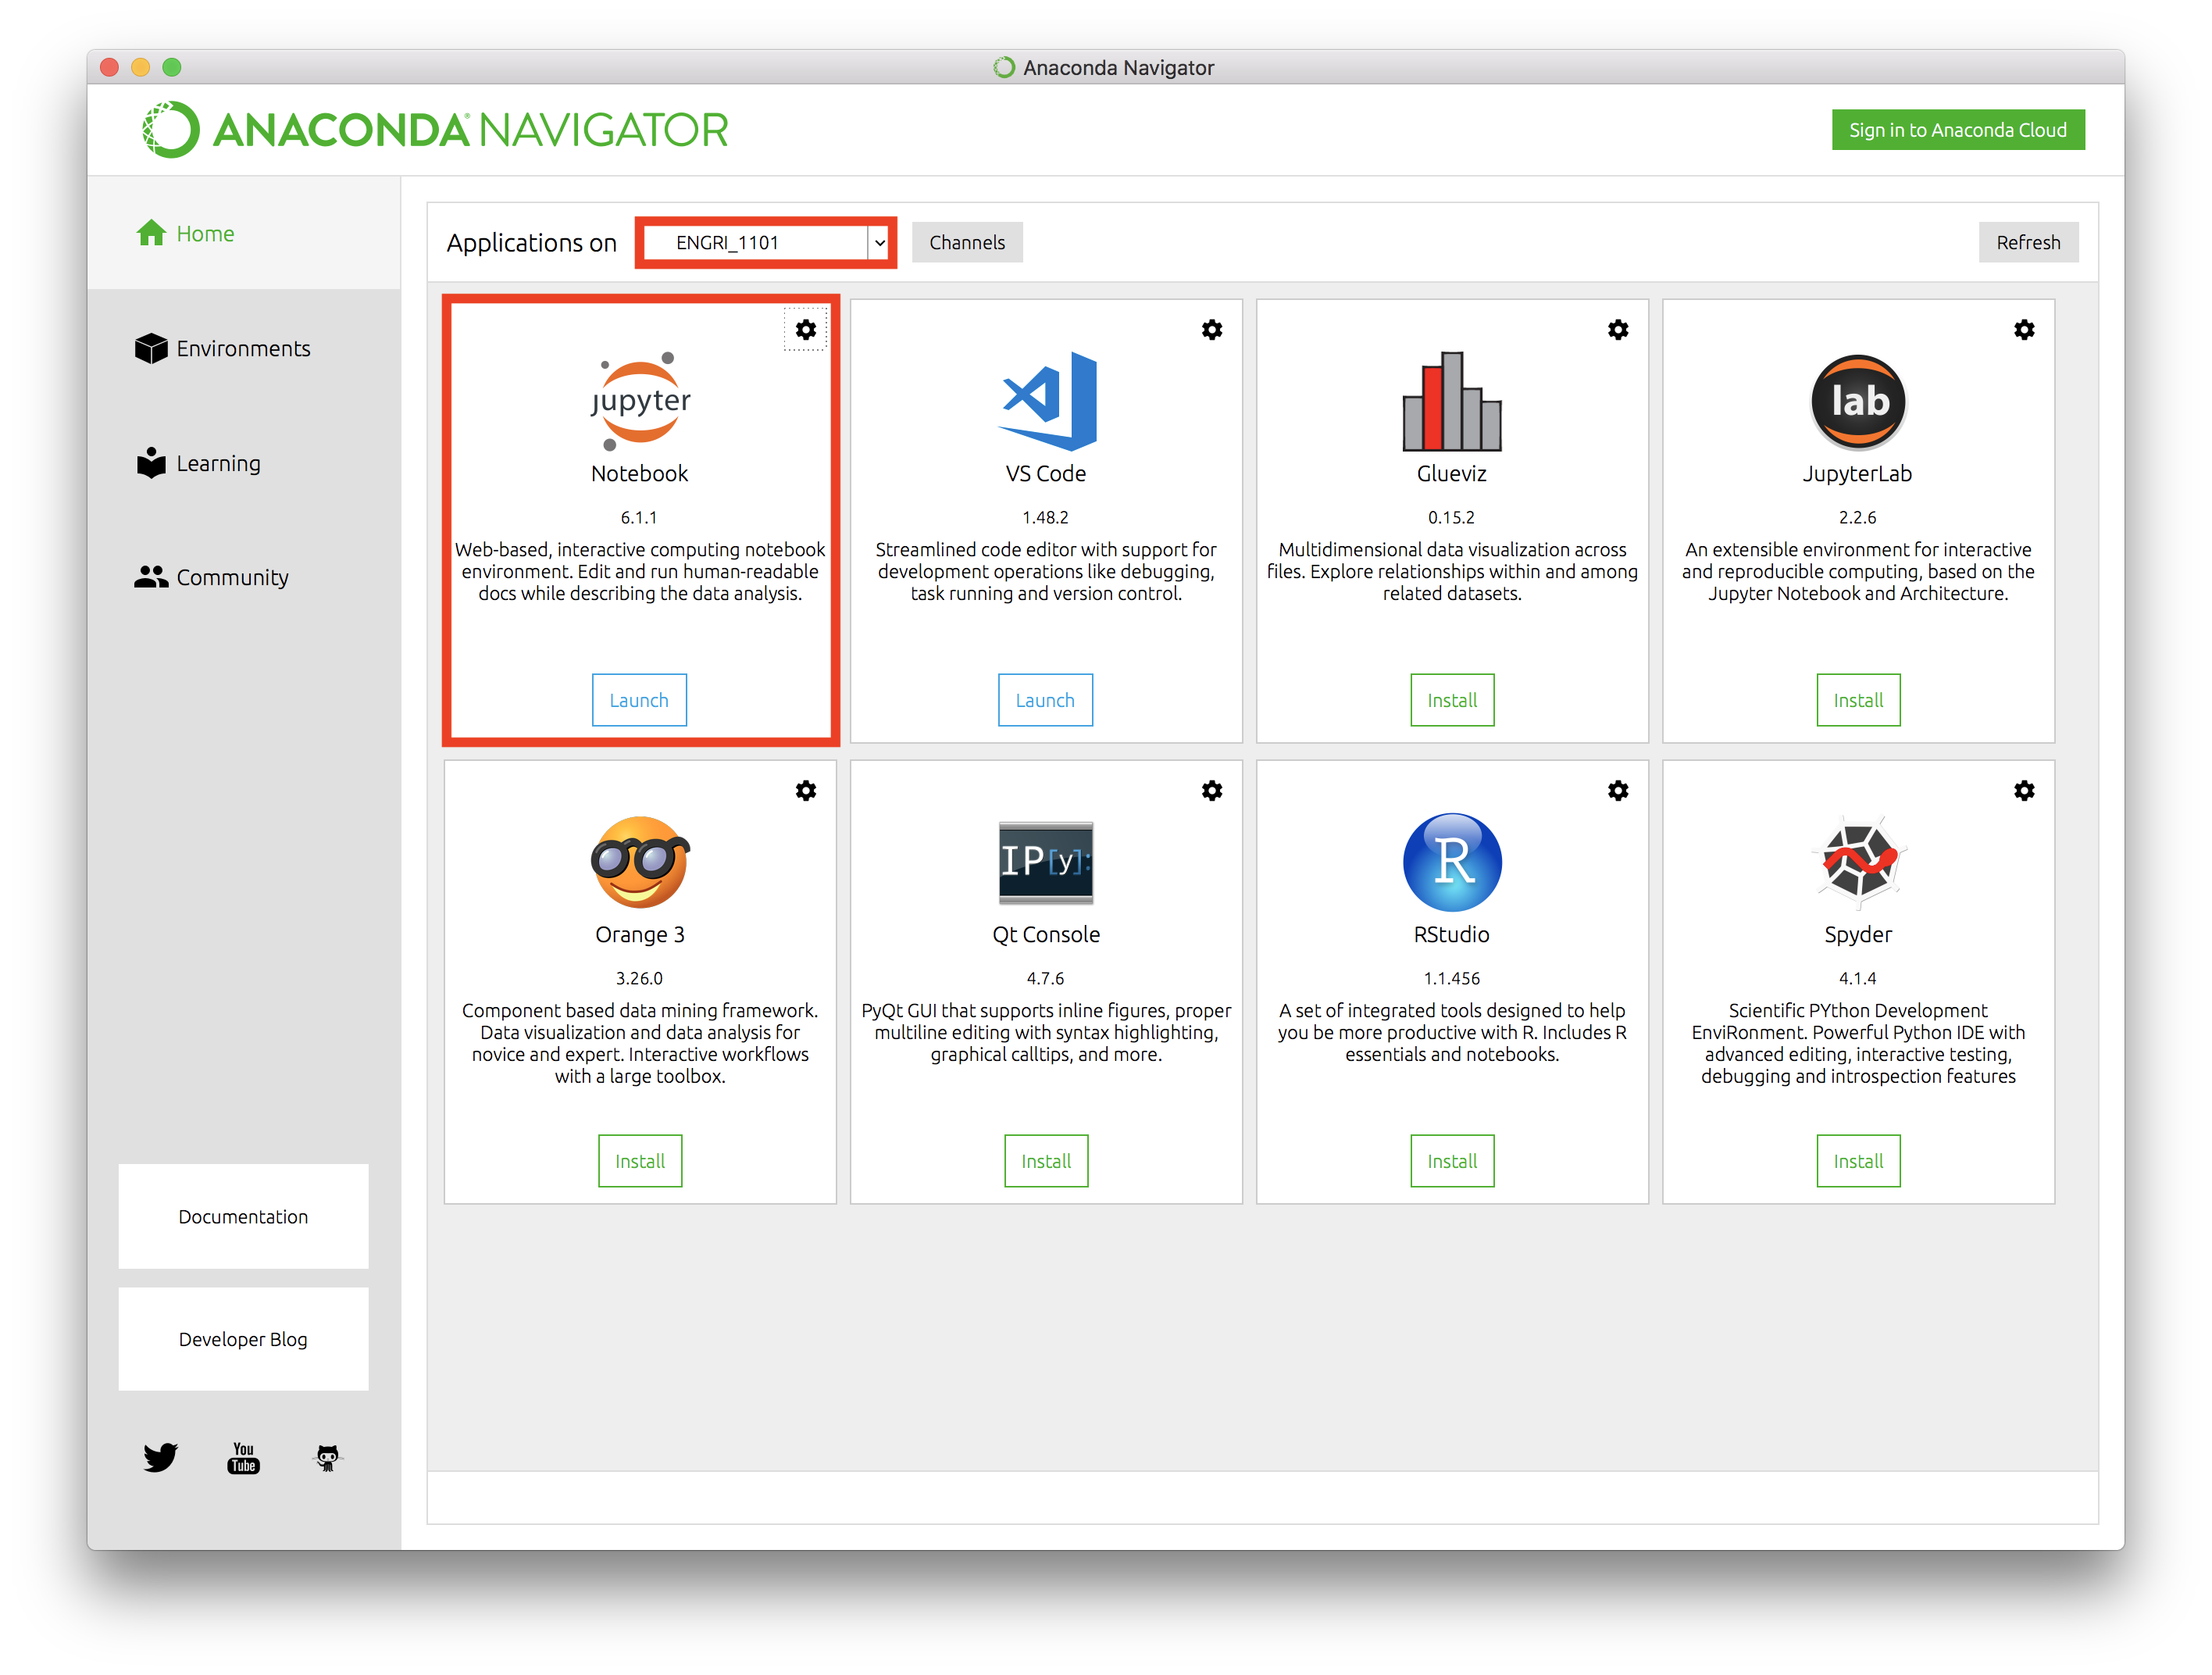
\includegraphics[scale=0.3]{install_jupyter}
\end{center}

\item Install \texttt{Jupyter Notebook}. Afterwards, you will be able to click \texttt{Launch} which will open up a web-browser tab displaying the home directory of your system. 

\item Navigate to the file \texttt{(START HERE) Test Install} and open it. Click the first block of code and then press \texttt{Run}. This should run without errors if your virtual environment has been set up properly!

\end{enumerate}

\section{Gurobi Installation}

The Python package \texttt{ortools} is Google's optimization suite. It contains an open-source linear program (LP) and integer linear program (ILP) solver. However, it can also serve as a way to interact with the cutting-edge Gurobi solver. In order to use solve LPs and ILPs in \texttt{ortools} using Gurobi, you will need to download additional software. First, you will create an \href{https://pages.gurobi.com/registration}{Academic User Account}. Next, download the \texttt{Gurobi Optimizer} found at \href{https://www.gurobi.com/downloads/}{Gurobi Downloads}. Lastly, you will need to create an academic license to use the software. Register for an \href{https://www.gurobi.com/downloads/end-user-license-agreement-academic/}{Academic License}. After generating your unique academic license, you will be given a line to run in your terminal. When prompted, select the default location for the license file.


\begin{center}
%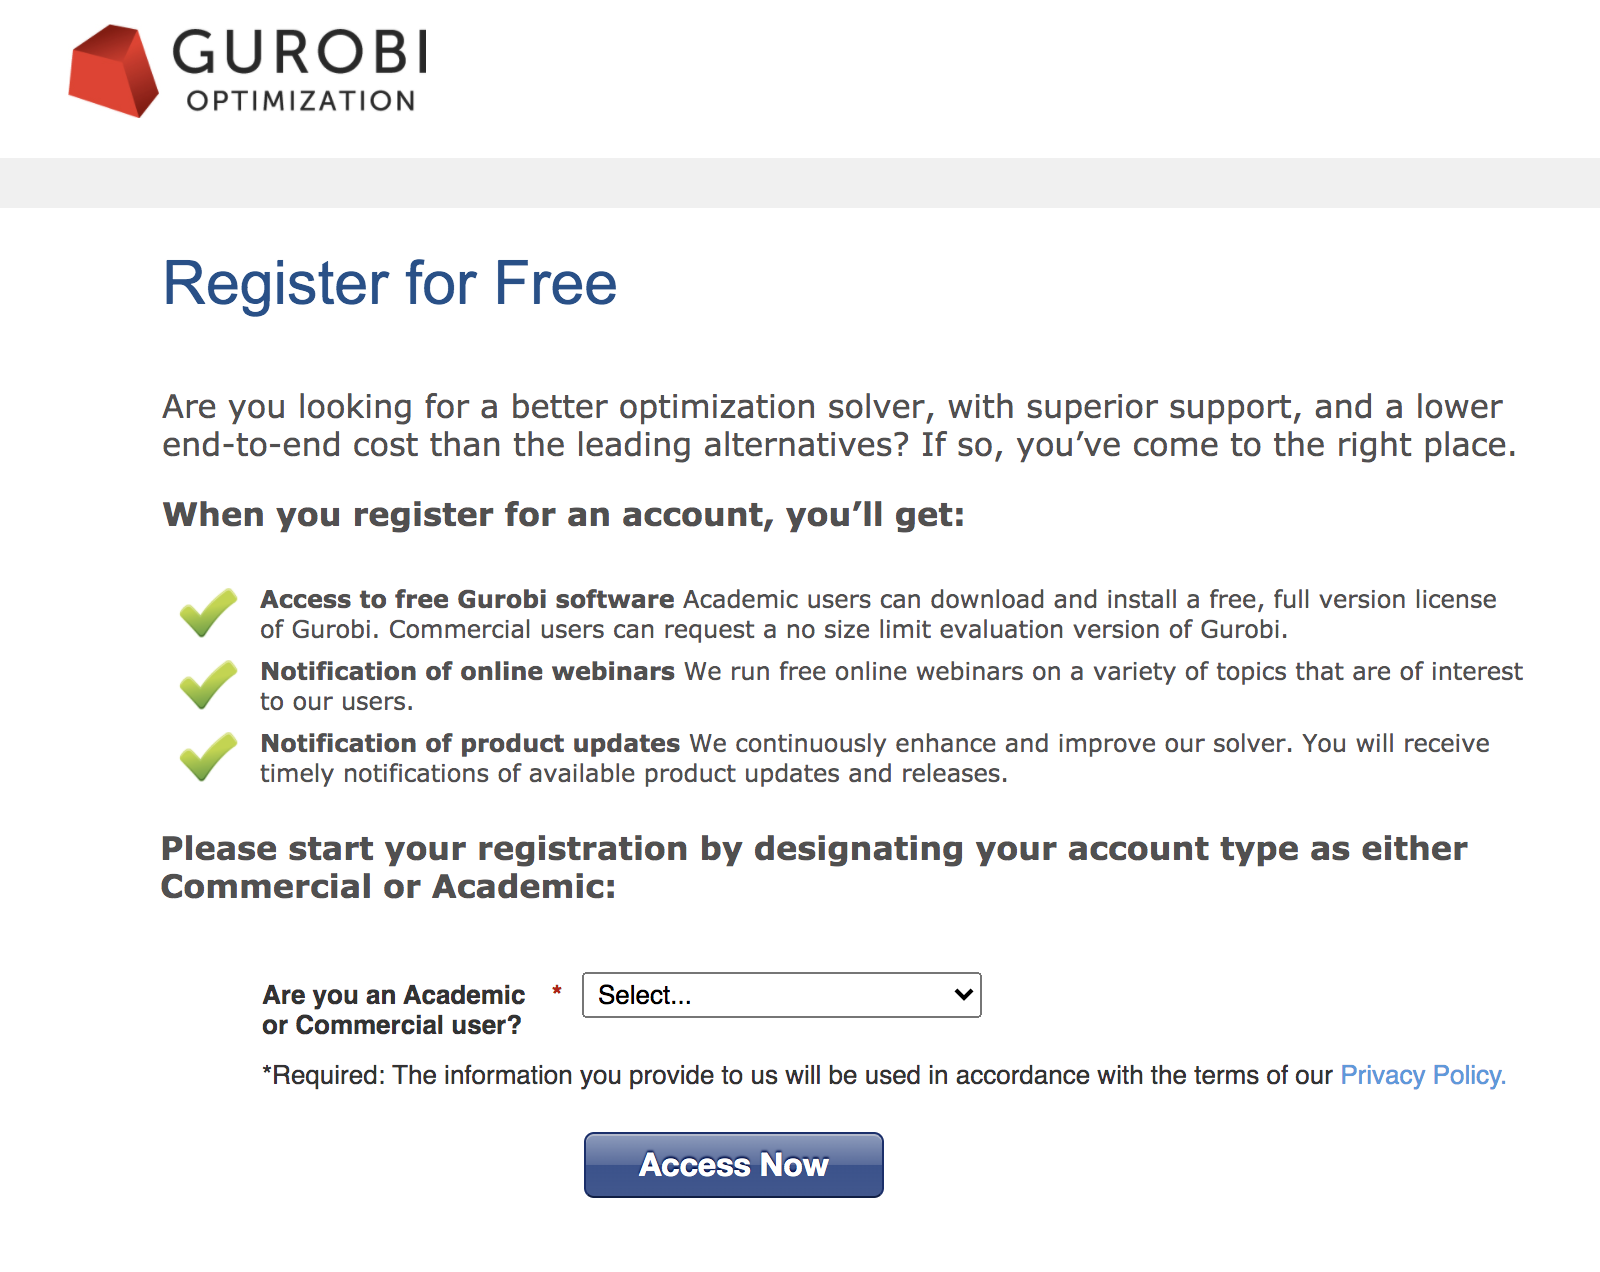
\includegraphics[scale=0.3]{gurobi_registration}
\end{center}
\begin{center}
%
\includegraphics[scale=0.3]{gurobi_download}
\end{center}


\end{document}